\chapter{OVERVIEW ITS SYSTEM}

\renewcommand{\headrulewidth}{0.5pt}
\renewcommand{\footrulewidth}{0.5pt}
\thispagestyle{plain}
\pagestyle{fancy}
\fancyhf{}
\fancyhead[L]{\textbf{CHAPTER 1}}
\fancyhead[R]{\textbf{Intelligent Traffic System}}
\raggedright
\fancyfoot[L]{From: ITM Vision}
\fancyfoot[R]{Page \thepage}

\section{ITS}
    Nowadays, Artificial Intelligence or AI for short have been widely embedded to urban management system, education management, medical, etc, 
    we may name a few of them: traffic analysis, security analysis, medical image processing, patient monitoring. \\ 
    \vspace{3mm}
    Applying AI to support decision making is an explosive trend from countries to countries, from Small-Medium Enterprise to Global Cooperation 
    therefore the fact that government leveraging AI for managing infrastructure and social activities is no exception. \\ 
    \vspace{3mm}
    Hangzhou City is a one of the most well-known pioneers for their success of cutting down traffic jam to the lowest level by taking advantage of 
    AI tools and platform, which takes video stream from crowded intersections and performs real-time analytics to optimize downtime due to traffic 
    flow congestion. \\ 
    \vspace{3mm}
    According to Vietnam Ministry of Information and Communications' Guidance for Integrating AI Platform to public infrastructure, developing 
    intelligent traffic system is urgent and encouraged toward transformation of big cities into smart cities. \\ 
    \vspace{3mm}
    Foundation of AI platform for Smart Traffic System includes:
    \begin{itemize}
        \item \textbf{Node Management:} Job orchestration for AI node in system.
        \item \textbf{Streaming:} Management and distribution of encoded data flown to AI node and metadata storage after analytics.
        \item \textbf{Blockchain:} Storage for machine to machine or human to machine transaction data such as: Authentication and Indexing AI model, Validation 
        of AI inference results, Events,etc.
        \item \textbf{Notification:} Event Management for operation of system as a whole including system notification, object detected notification, etc.
        \item \textbf{Training:} Data mining, training AI models and updating weights and architecture of AI models.
        \item \textbf{Marketplace:} Managing, Publish, Exchange AI models.
        \item \textbf{AI Brain:}
            \begin{itemize}
                \item \textbf{AI inference engine:} Creating data pipeline, feature extractions and AI inference.
                \item \textbf{AI rule base configuration:} Threshold configuration for decision making based on AI inference results.
            \end{itemize}
        \item \textbf{Storage:} Raw data and metadata storage after analytics.
    \end{itemize}
    Level of AI integration to infrastructure:
    \begin{itemize}
        \item \textbf{Level 1:} Objects Detection. At this level, AI applications are able to detect objects according to supplied labels.
        \item \textbf{Level 2a:} Object Recognition. AI processes abilities to distinguish different object instances belonging to same class of label.
        \item \textbf{Level 2b:} Object Tracking. AI applications at this level are capable of generating tracklet of detected instances of specific 
        class from level 1 application or 2a.
        \item \textbf{Level 3:} Behavior Recognition. In order to reach level 3, AI application must show enormous inference performance in tracking 
        multi objects and predicting their behavior at a same time. 
    \end{itemize}
    \begin{figure}[H]
        \centering
        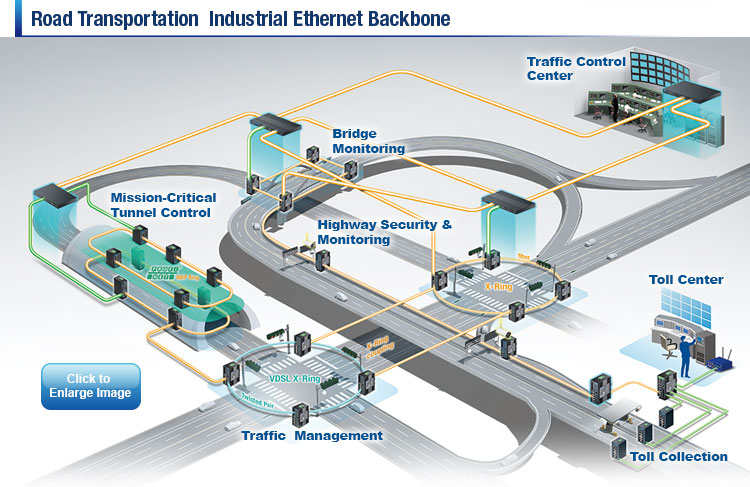
\includegraphics[width=0.6\linewidth]{img/ITS.png}
        \caption{Some components of AI node in ITS}
    \end{figure}

\section{Jetson Platform}

    \subsection{Introduction}
        NVIDIA \textregistered Jetson \texttrademark is the world's leading platform for AI at the edge. 
        Its high-performance, low-power computing for \textbf{deep learning} and computer vision makes it the ideal 
        platform for compute-intensive projects. The Jetson platform includes a variety of Jetson modules 
        together with NVIDIA JetPack \texttrademark SDK. \\ 
        \vspace{3mm}
        Each \textbf{Jetson module} is a computing system packaged as a plug-in unit (System on Module). NVIDIA offers a 
        variety of Jetson modules with different capabilities. \\ 
        \vspace{3mm}
        \textbf{JetPack} bundles all of the Jetson platform software, starting with the NVIDIA \textregistered Jetson \texttrademark 
        Linux Driver Package (L4T).L4T provides the Linux kernel, bootloader, NVIDIA drivers, flashing utilities, sample filesystem, 
        and more for the Jetson platform.
    \subsection{Jetson Developer Kits and Modules}
        \textbf{Jetson Developer Kits} include a non-production specification Jetson module attached to a reference carrier board. 
        Together with \textbf{JetPack SDK}, it is used to develop and test software for your use case. Jetson developer kits are not intended 
        for production use. \\ 
        \vspace{3mm}
        Jetson modules are suitable for deployment in a production environment throughout their operating lifetime. Each Jetson module ships 
        with no software pre-installed; you attach it to a carrier board designed or procured for your end product, and flash it with the software 
        image you’ve developed.
    \subsection{Jetson Nano}
        NVIDIA announced the \textbf{Jetson Nano Developer Kit} at the 2019 NVIDIA GPU Technology Conference (GTC) available now for embedded designers, 
        researchers, and DIY makers, delivering the power of modern AI in a compact, easy-to-use platform with full software programmability. Jetson Nano 
        delivers 472 GFLOPS of compute performance with a quad-core 64-bit ARM CPU and a 128-core integrated NVIDIA GPU. It also includes 4GB LPDDR4 memory 
        in an efficient, low-power package with 5W/10W power modes and 5V DC input.
        \begin{figure}[H]
            \centering
            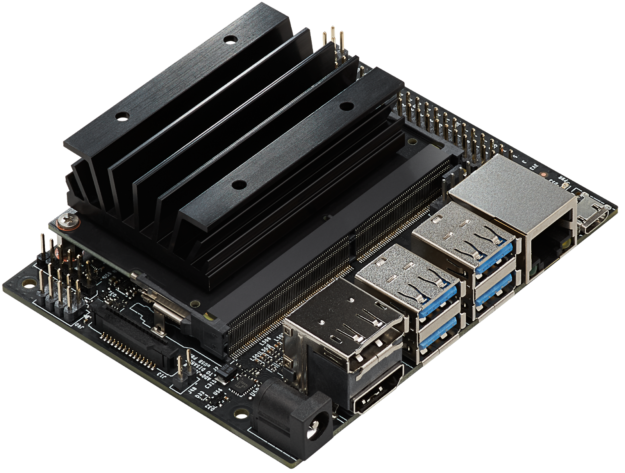
\includegraphics[width=0.6\linewidth]{img/jetson_nano.png}
            \caption{Jetson Developer Kit (80x100mm)}
        \end{figure}
        They newly released \textbf{Jetpack 4.2 SDK} provides a complete desktop Linux environment for Jetson Nano based on Ubuntu 18.04 with accelerated graphics, 
        support for NVIDIA CUDA Toolkit 10.0, and libraries such as cuDNN 7.3 and TensorRT 5.The SDK also includes the ability to natively install popular open source 
        Machine Learning (ML) frameworks such as TensorFlow, PyTorch, Caffe, Keras, and MXNet, along with frameworks for computer vision and robotics development like OpenCV and ROS. \\ 
        \vspace{3mm}
        Full compatibility with these frameworks and NVIDIA’s leading AI platform makes it easier than ever to deploy AI-based inference workloads to Jetson. Jetson Nano brings real-time 
        computer vision and inferencing across a wide variety of complex Deep Neural Network (DNN) models.
        \begin{figure}[H]
            \centering
            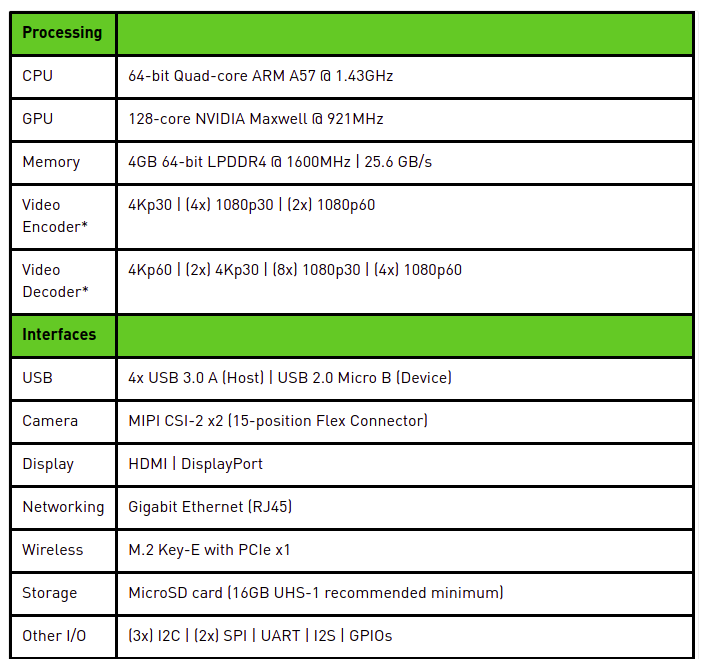
\includegraphics[width=0.6\linewidth]{img/nano-kit.png}
            \caption{Jetson Nano Developer Kit technical specifications}
        \end{figure}
        The devkit is built around a 260-pin SODIMM-style System-on-Module (SoM). The SoM contains the processor, memory, and power management circuitry. The production compute module will 
        include 16GB eMMC onboard storage and enhanced I/O with PCIe Gen2 x4/x2/x1, MIPI DSI, additional GPIO, and 12 lanes of MIPI CSI-2 for connecting up to three x4 cameras or up to four 
        cameras in x4/x2 configurations. Jetson’s unified memory subsystem, which is shared between CPU, GPU, and multimedia engines, provides streamlined ZeroCopy sensor ingest and efficient 
        processing pipelines.
        \begin{figure}[H]
            \centering
            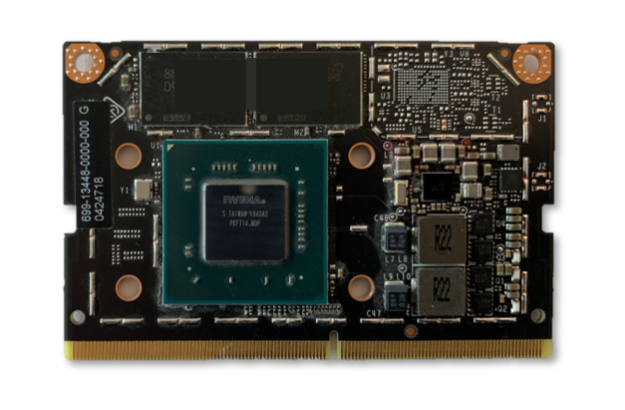
\includegraphics[width=0.6\linewidth]{img/nano-compute.png}
            \caption{45x70mm Jetson Nano compute module with 260-pin edge connector}
        \end{figure}
        \subsubsection{Deep Learning Inference Benchmarks}
            Jetson Nano can run a wide variety of advanced networks, including the full native versions of popular ML frameworks like TensorFlow, PyTorch, Caffe/Caffe2, Keras, MXNet, and others. 
            These networks can be used to build autonomous machines and complex AI systems by implementing robust capabilities such as image recognition, object detection and localization, pose 
            estimation, semantic segmentation, video enhancement, and intelligent analytics. \\ 
            \vspace{3mm}
            The inferencing used batch size 1 and FP16 precision, employing NVIDIA’s \textbf{TensorRT} accelerator library included with JetPack 4.2. Jetson Nano attains real-time performance in many 
            scenarios and is capable of processing multiple high-definition video streams.
            \begin{figure}[H]
                \centering
                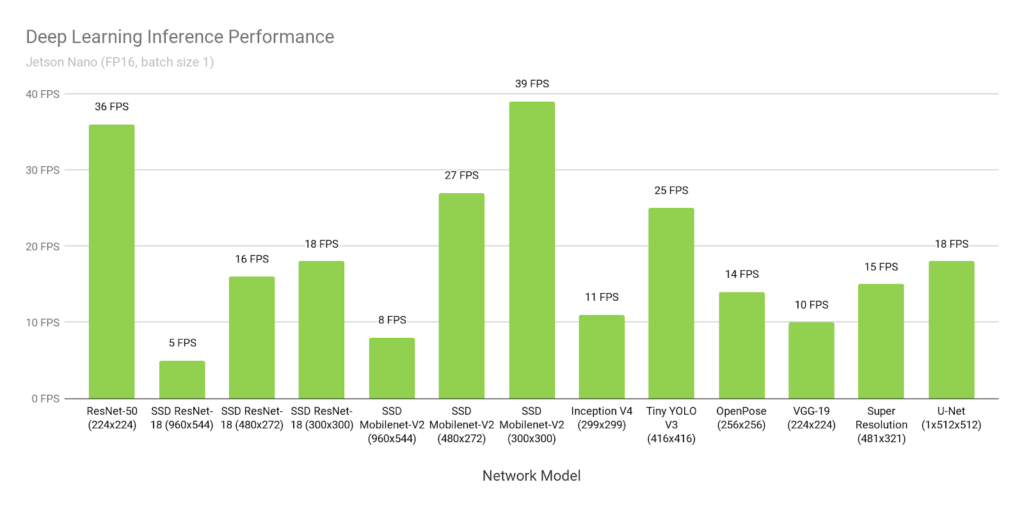
\includegraphics[width=0.6\linewidth]{img/jetson-nano-inference.png}
                \caption{Performance of various deep learning inference networks with Jetson Nano and TensorRT}
            \end{figure}
        \subsubsection{Multi-Stream Video Analytics}
            Jetson Nano processes up to eight HD full-motion video streams in real-time and can be deployed as a low-power edge intelligent video analytics platform for Network Video Recorders (NVR), 
            smart cameras, and IoT gateways. NVIDIA’s \textbf{DeepStream SDK} optimizes the end-to-end inferencing pipeline with ZeroCopy and TensorRT to achieve ultimate performance at the edge and for on-premises 
            servers. The video below shows Jetson Nano performing object detection on eight 1080p30 streams simultaneously with a ResNet-based model running at full resolution and a throughput of 500 
            megapixels per second (MP/s).
            \begin{figure}[H]
                \centering
                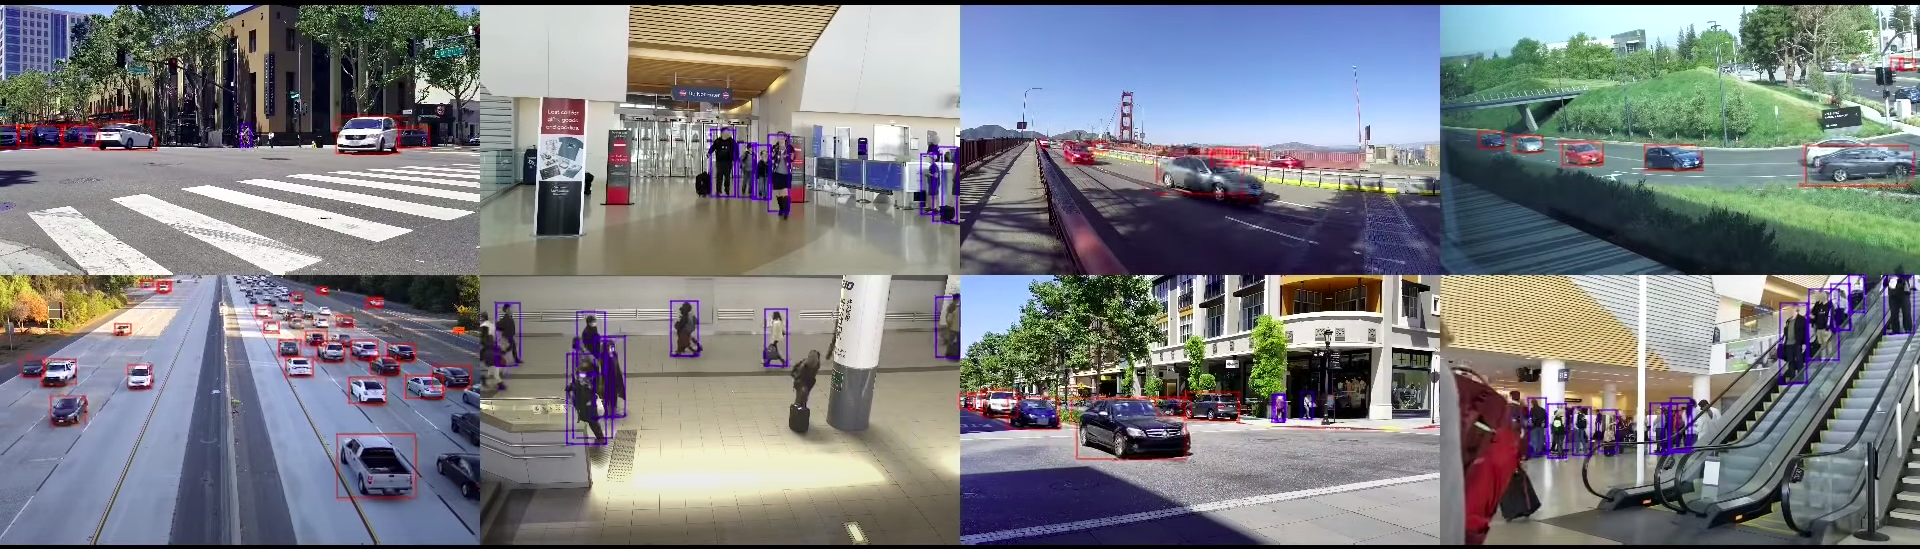
\includegraphics[width=0.6\linewidth]{img/deep-stream.png}
                \caption{DeepStream application running on Jetson Nano with ResNet-based object detector concurrently on eight independent 1080p30 video streams}
            \end{figure}
            \begin{figure}[H]
                \centering
                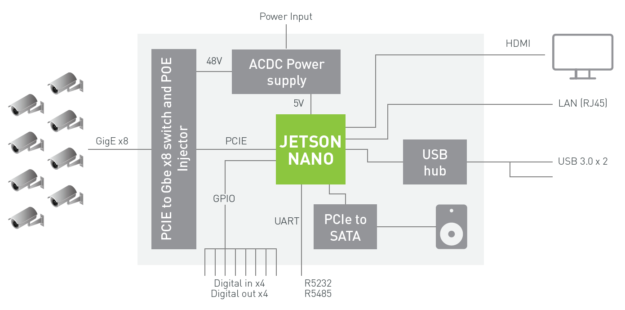
\includegraphics[width=0.6\linewidth]{img/NVR.png}
                \caption{Reference NVR system architecture with Jetson Nano and 8x HD camera inputs}
            \end{figure}
            This figure shows an example NVR architecture using Jetson Nano for ingesting and processing up to eight digital streams over Gigabit Ethernet with deep learning analytics. The system can decode 500 MP/s 
            of H.264/H.265 and encode 250 MP/s of H.264/H.265 video.
    \subsection{Jetson TX1}
        It's a small form-factor Linux system-on-module, destined for demanding embedded applications in visual computing. Designed for developers and makers everywhere, the miniature Jetson TX1 deploys teraflop-level 
        supercomputing performance onboard platforms in the field. Backed by the Jetson TX1 Developer Kit, a premier developer community, and a software ecosystem including Jetpack, Linux For Tegra R23.1, CUDA Toolkit 7, 
        cuDNN, and VisionWorks. \\ 
        \vspace{3mm}
        Jetson TX1’s credit-card footprint and low power consumption mean that it’s geared for deployment onboard embedded systems with constrained size, weight, and power (SWaP). Jetson TX1 exceeds the performance of 
        Intel’s high-end Core i7-6700K Skylake in deep learning classification with Caffe, and while drawing only a fraction of the power, achieves more than ten times the perf-per-watt.
        \subsubsection{Jetson TX1 Module}
            Built around NVIDIA’s 20nm Tegra X1 SoC featuring the 1024-GFLOP Maxwell GPU, 64-bit quad-core ARM Cortex-A57, and hardware H.265 encoder/decoder, Jetson TX1 measures in at 50x87mm and is packed with performance 
            and functionality. Onboard components include 4GB LPDDR4, 16GB eMMC flash, 802.11ac WiFi, Bluetooth 4.0, Gigabit Ethernet, and accepts 5.5V-19.6VDC input. Peripheral interfaces consist of up to six MIPI CSI-2 cameras 
            (on a dual ISP), 2x USB 3.0, 3x USB 2.0, PCIe gen2 x4 + x1, independent HDMI 2.0/DP 1.2 and DSI/eDP 1.4, 3x SPI, 4x I2C, 3x UART, SATA, GPIO, and others. Needless to say, Jetson TX1 stands tall in the face of many an 
            algorithmic and integration challenge.
            \begin{figure}[H]
                \centering
                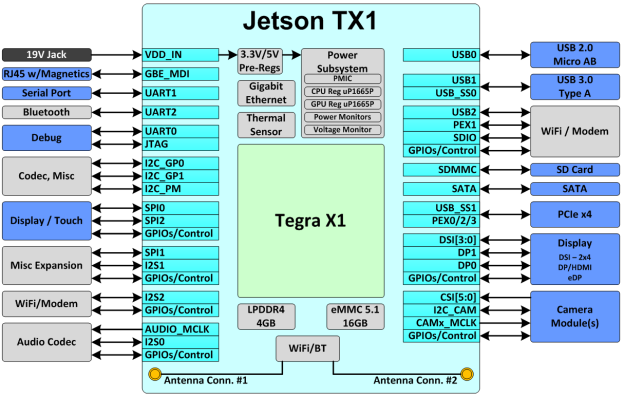
\includegraphics[width=0.6\linewidth]{img/TX1.png}
                \caption{Jetson TX1 block diagram}
            \end{figure}The Jetson module utilizes a 400-pin board-to-board connector for interfacing with the Developer Kit’s reference carrier board, or with a bespoke, customized board designed during your productization process. 
            Tegra’s chip-level capabilities and I/O are closely mapped to the module’s pin-out. The pin-out will be backward-compatible with future versions of the Jetson module. Jetson TX1 comes with an integrated thermal transfer 
            plate, rated between -25°C and 80°C, for interfacing with passive or active cooling solutions. Consult NVIDIA’s Embedded Developer Zone for thorough documentation and detailed electromechanical specifications, in addition 
            to visiting the active and open development community on Devtalk.
            \begin{figure}[H]
                \centering
                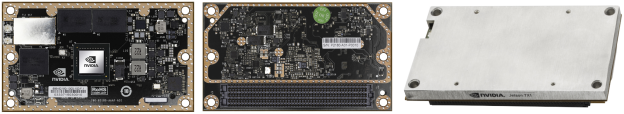
\includegraphics[width=0.6\linewidth]{img/structure.png}
                \caption{Left to right: Top of Jetson TX1 module, bottom (with connector), and complete assembly with TTP}
            \end{figure}
            Jetson TX1 draws as little as 1 watt of power or lower while idle, around 8-10 watts under typical CUDA load, and up to 15 watts TDP when the module is fully utilized, for example during gameplay and the most demanding vision routines. 
            Jetson TX1 provides exceptional dynamic power scaling either based on workload via its automated governor, or by explicit user commands to gate cores and specify clock frequencies. The four ARM A57 cores automatically scale between 102 MHz 
            and 1.9 GHz, the memory controller between 40MHz and 1.6GHz, and the Maxwell GPU between 76 MHz and 998 MHz. Touting 256 CUDA cores with Compute Capability 5.3 and Dynamic Parallelism, Jetson TX1’s Maxwell GPU is rated for up to 1024 GFLOPS 
            of FP16. When combined with support for up to 1200 megapixels/sec from either three MIPI CSI x4 cameras or six CSI x2 cameras, along with hardware H.265 encoder \& decoder, integrated WiFi and HDMI 2.0, Jetson TX1 is primed for all-4K video processing.
        \subsubsection{Jetson TX1 Developer Kit}
            The Jetson TX1 Developer Kit contains a reference mini-ITX carrier board, 5MP MIPI CSI-2 camera module, two 2.4/5GHz antennas, an active heatsink \& fan, an acrylic base plate, and a 19VDC power supply brick.
            \begin{figure}[H]
                \centering
                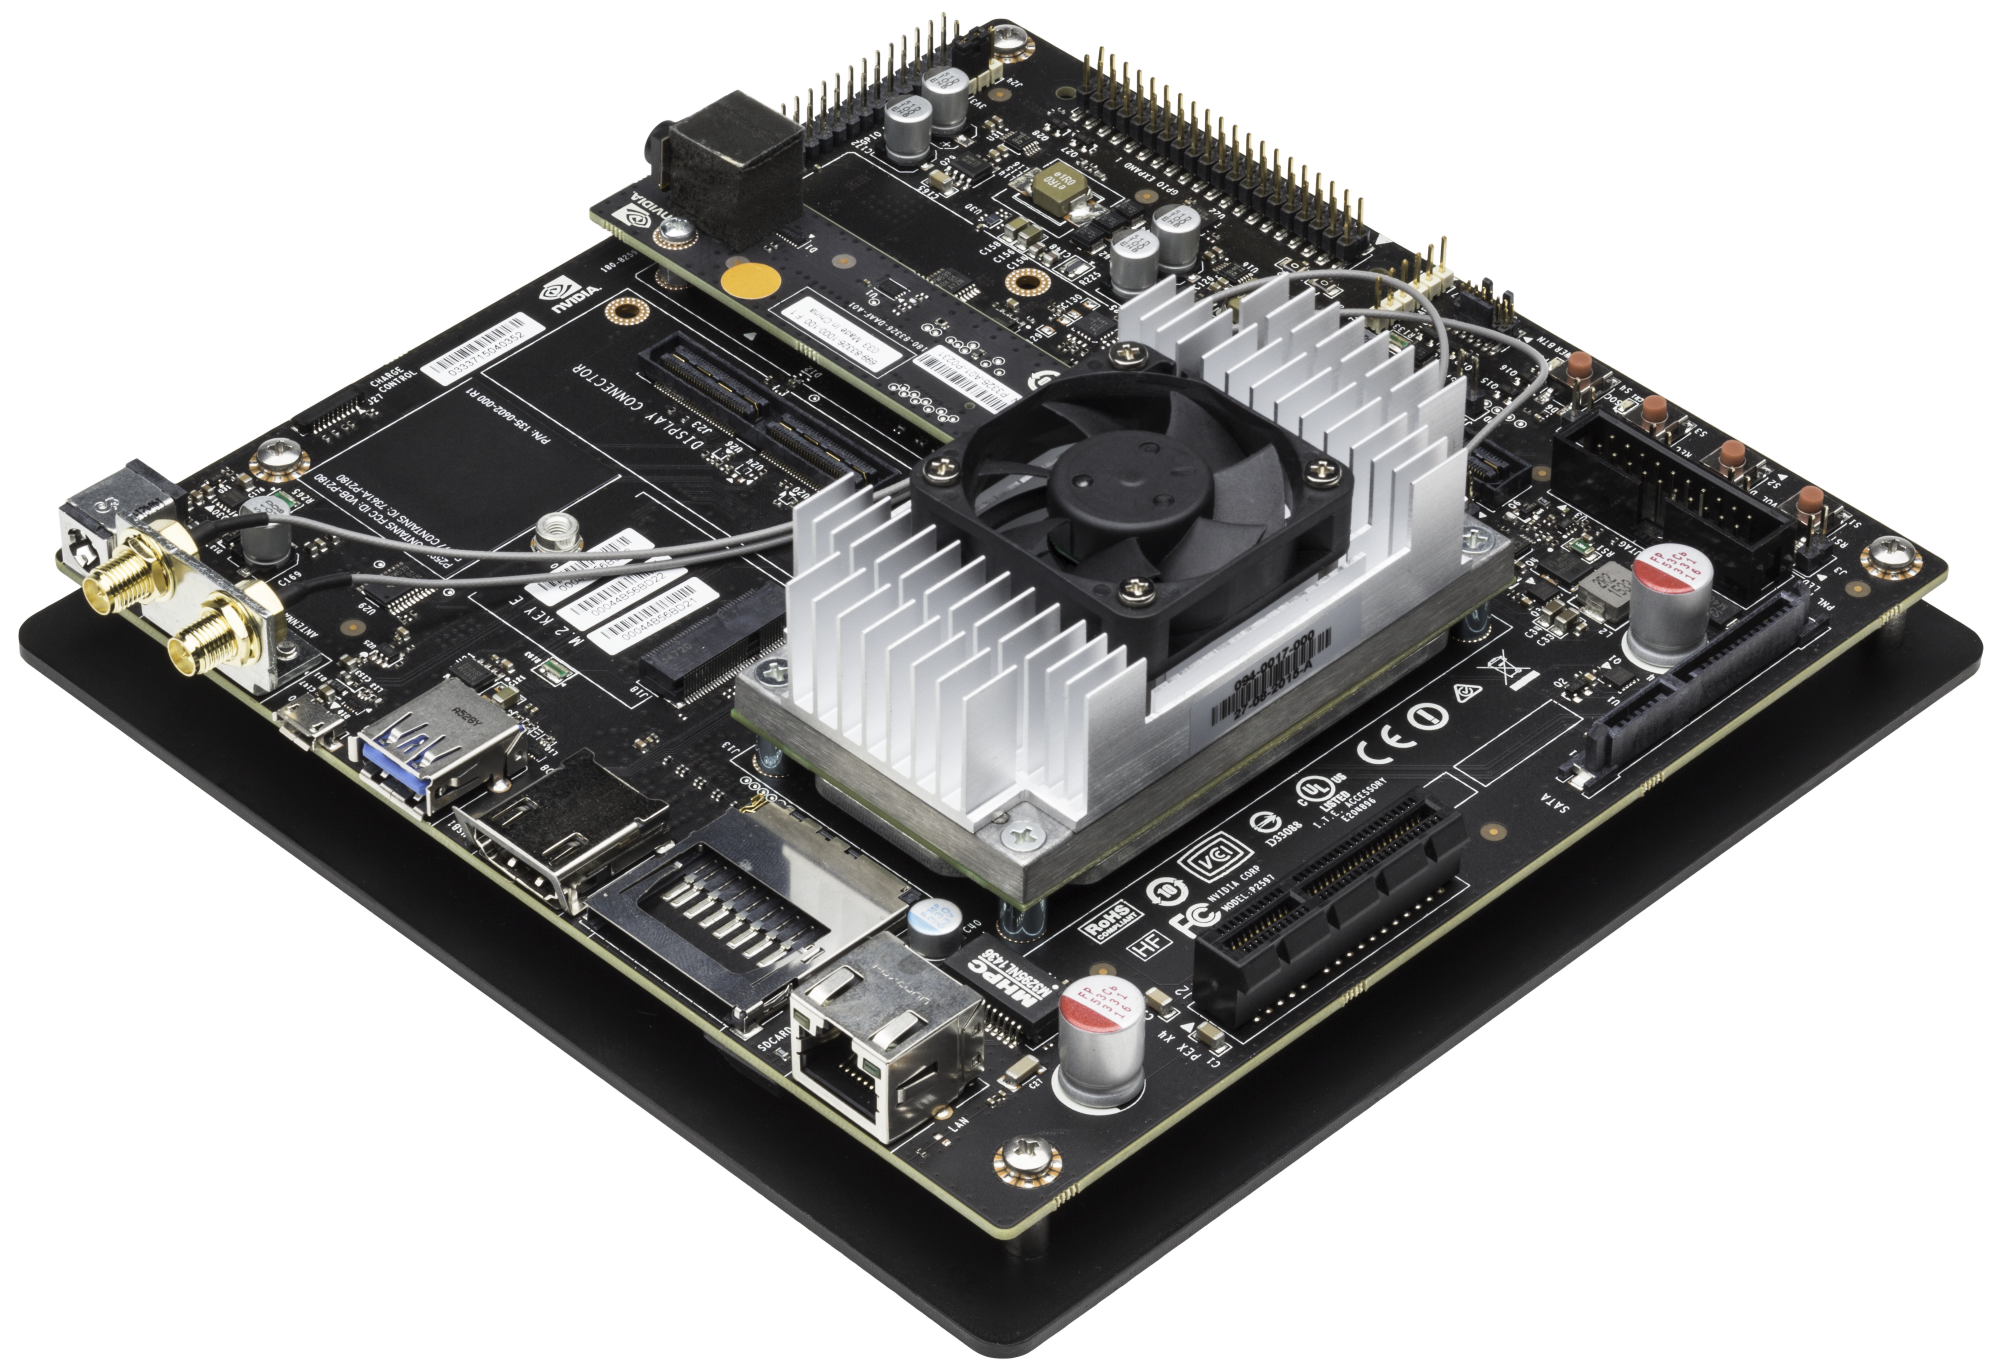
\includegraphics[width=0.6\linewidth]{img/tx1-dev-kit.png}
                \caption{Jetson TX1 Developer Kit, including module, reference carrier and camera board}
            \end{figure}
            The PCIe lanes on the Jetson TK1 Developer Kit are routed from the module to a PCIe x4 desktop slot on the carrier for easy prototyping, in addition to an M.2-E mezzanine with PCIe x1 for wireless radios. Available on the Embedded Developer Zone, 
            NVIDIA shares the schematics and design files for the reference carrier along with the 5MP CSI-2 camera module, including routing and signal integrity guidelines. Board software support bundled by Jetpack provides easy flashing and device configuration. 
            Out of the box, the Jetson TX1 Developer Kit provides the experience of a desktop PC, but in a small embedded form factor that only draws a fraction of the power.
        \subsubsection{Vision Works}
            Jetson TX1 marks the first release of VisionWorks available to developers through Jetpack 2.0 and the \textbf{Embedded Developer Zone}. VisionWorks provides primitives and building blocks that are highly optimized for Tegra using tuned CUDA kernels.
            \begin{figure}[H]
                \centering
                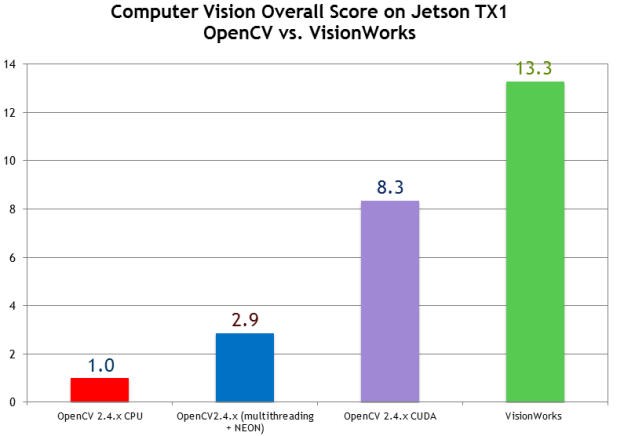
\includegraphics[width=0.6\linewidth]{img/tx1-benchmark.png}
                \caption{Benchmarks demonstrate the large speedup of VisionWorks vs. OpenCV running on the Jetson TX1 CPU and GPU}
            \end{figure}
            VisionWorks is more than 10x faster than upstream CPU-only OpenCV, is 4.5x faster than OpenCV4Tegra with NEON extensions, and is 1.6x faster than OpenCV’s GPU module. The Overall Computer Vision Score was collected from the geometric mean performance 
            of all the overlapping primitives between OpenCV and VisionWorks. Each primitive was measured across image sizes 720p and larger, and across all permutations of argument parameters. \\ 
            \vspace{3mm}
            In addition to more than 50 filtering, warping, and image-enhancement primitives, VisionWorks also offers numerous higher-level building blocks as well, such as LK optical flow, stereo block-matching (SBM), Hough lines \& circles, and Harris (Corner) 
            feature-detection \& tracking. VisionWorks provides a full implementation of OpenVX 1.1. Developers can leverage VisionWorks to deploy camera-ready algorithms and vision pipelines, already tuned for Jetson.
        \subsubsection{Development Platforms}
            The NVIDIA Jetson ecosystem is rich with tools and support for enabling your research and development of applications and products with Jetson TX1. In the larger scheme, NVIDIA software toolkits for accelerated computing, deep learning, computer vision, 
            and graphics are portable from the datacenter to the workstation to embedded SoC, allowing enterprise users to seamlessly scale and deploy their applications to devices in the field. Using Jetson, developers can leverage NVIDIA’s shared architecture and 
            power-efficient technology to roll out high-performance embedded systems with ease and flexibility.
            \begin{figure}
                \centering
                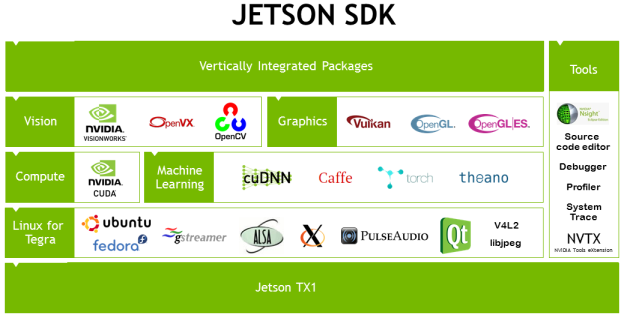
\includegraphics[width=0.6\linewidth]{img/jetson-sdk.png}
                \caption{Jetson taps into the NVIDIA ecosystem to deliver unprecedented scalability and developer-friendly support}
            \end{figure}
    \subsection{Jetson TX2}
        Jetson is the world’s leading low-power embedded platform, enabling server-class AI compute performance for edge devices everywhere. Jetson TX2 features an integrated 256-core NVIDIA Pascal GPU, a hex-core ARMv8 64-bit CPU complex, and 8GB of LPDDR4 memory with 
        a 128-bit interface. The CPU complex combines a dual-core NVIDIA Denver 2 alongside a quad-core Arm Cortex-A57. The Jetson TX2 module fits a small Size, Weight, and Power (SWaP) footprint of 50 x 87 mm, 85 grams, and 7.5 watts of typical energy usage.
        \begin{figure}[H]
            \centering
            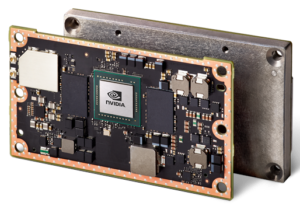
\includegraphics[width=0.6\linewidth]{img/tx2.png}
            \caption{NVIDIA Jetson TX2 embedded system-on-module with Thermal Transfer Plate (TTP)}
        \end{figure}
        Internet-of-Things (IoT) devices typically function as simple gateways for relaying data. They rely on cloud connectivity to perform their heavy lifting and number-crunching. Edge computing is an emerging paradigm which uses local computing to enable analytics at 
        the source of the data. With more than a TFLOP/s of performance, Jetson TX2 is ideal for deploying advanced AI to remote field locations with poor or expensive internet connectivity. Jetson TX2 also offers near-real-time responsiveness and minimal latency—key for 
        intelligent machines that need mission-critical autonomy.
        Jetson TX2 is based on the 16nm NVIDIA Tegra “Parker” system on a chip (SoC). Jetson TX2 is twice as energy efficient for \textbf{Deep Learning} inference than its predecessor, Jetson TX1, and offers higher performance than an Intel Xeon Server CPU. This jump in efficiency 
        redefines possibilities for extending advanced AI from the cloud to the edge.
        \begin{figure}[H]
            \centering
            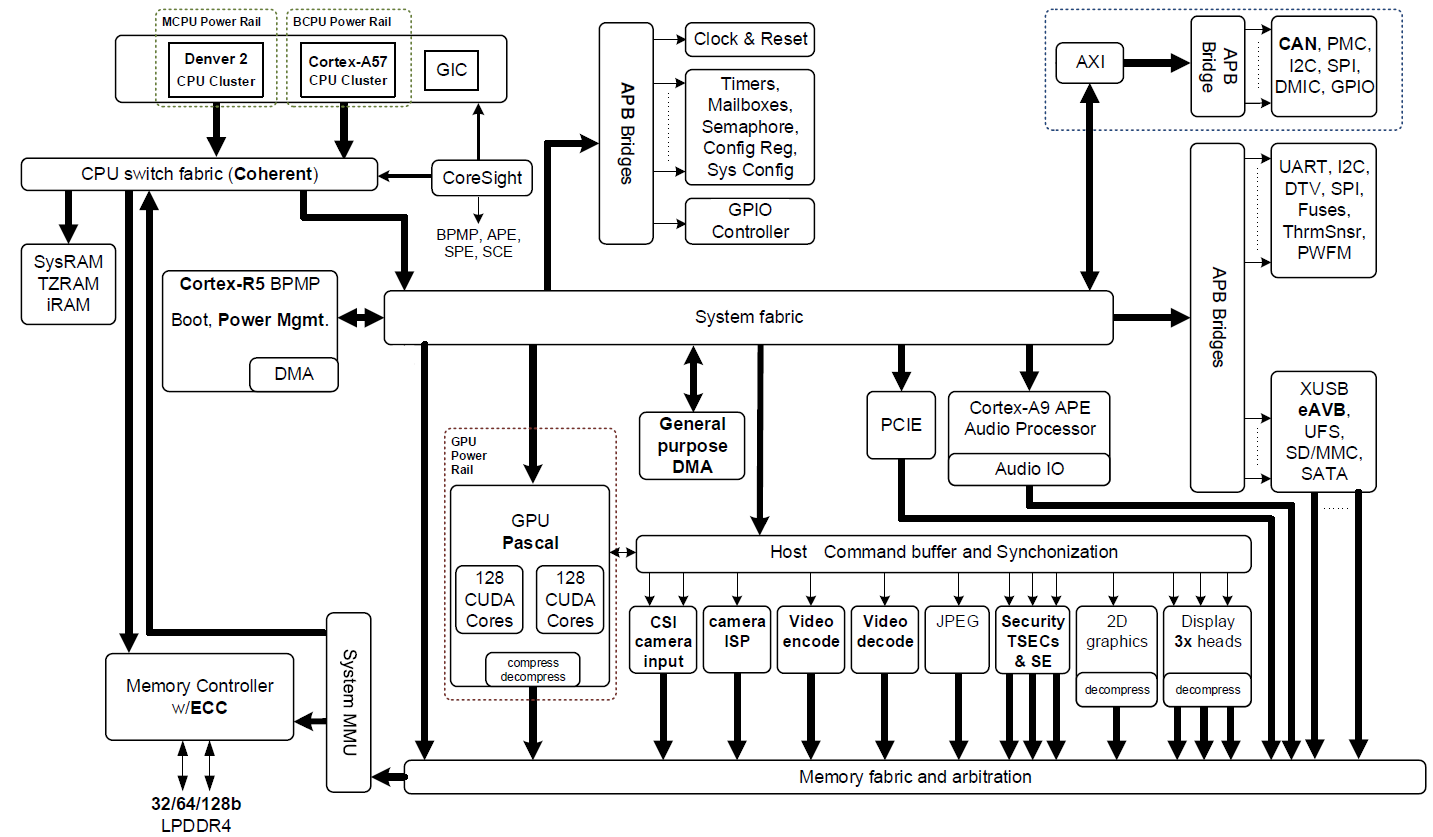
\includegraphics[width=0.6\linewidth]{img/tegra.png}
            \caption{NVIDIA Jetson TX2 Tegra “Parker” SoC block diagram featuring integrated NVIDIA Pascal GPU, NVIDIA Denver 2 + Arm Cortex-A57 CPU clusters, and multimedia acceleration engines}
        \end{figure}
        Jetson TX2 has multiple multimedia streaming engines to keep its Pascal GPU fed with data by offloading sensor acquisition and distribution. These multimedia engines include six dedicated MIPI CSI-2 camera ports that provide up to 2.5 Gb/s per lane of bandwidth and 1.4 
        gigapixels/s processing by dual Image Service Processors (ISP), as well as video codecs supporting H.265 at 4K 60 frames per second. \\ 
        \vspace{3mm}
        Jetson TX2 accelerates cutting-edge deep neural network (DNN) architectures using the NVIDIA cuDNN and TensorRT libraries, with support for \textbf{Recurrent Neural Networks (RNNs)}, \textbf{Long Short-Term Memory networks (LSTMs)}, and online \textbf{Reinforcement Learning}. Its dual-CAN bus 
        controller enables autopilot integration to control robots and drones that use DNNs to perceive the world around them and operate safely in dynamic environments. Software for Jetson TX2 is provided through NVIDIA’s JetPack 3.0 and Linux For Tegra (L4T) Board Support Package (BSP).
        \begin{figure}[H]
            \centering
            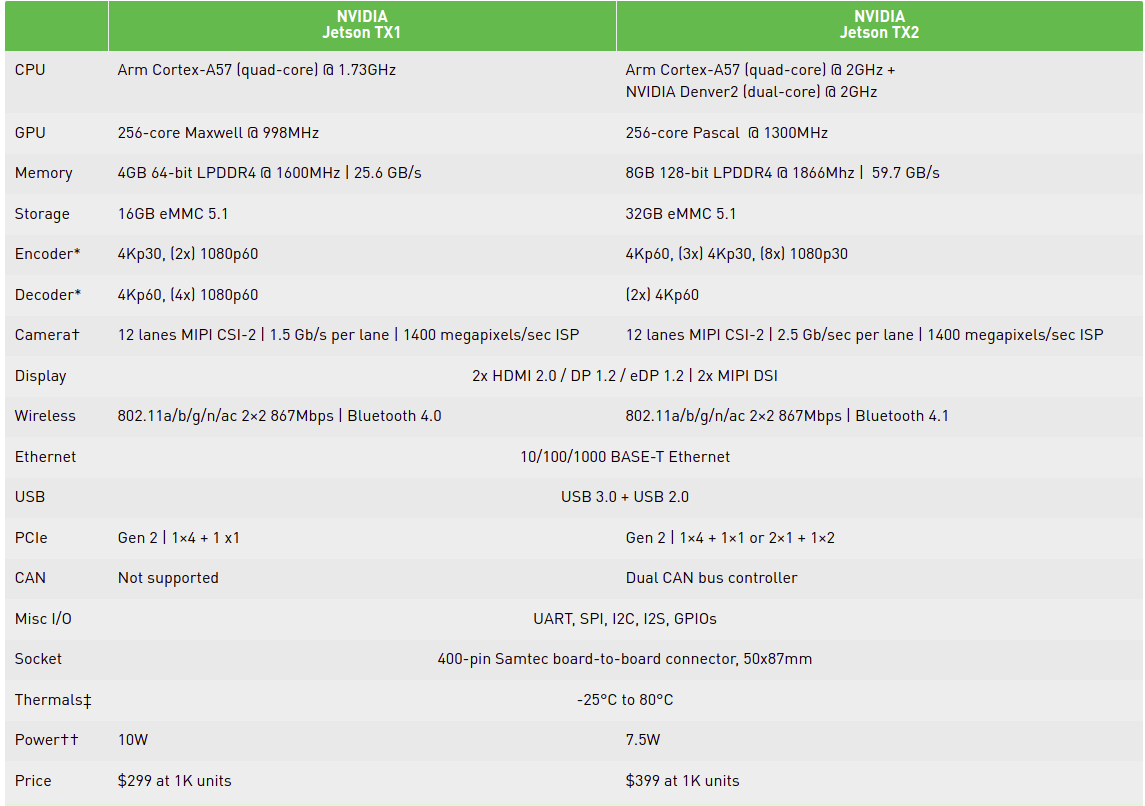
\includegraphics[width=0.6\linewidth]{img/comparision.png}
            \caption{Comparison of Jetson TX1 and Jetson TX2}
        \end{figure}
        \subsubsection{Twice the Performance, Twice the Efficiency}
            TensorRT optimizes production networks to significantly improve performance by using graph optimizations, kernel fusion, half-precision floating point computation (FP16), and architecture autotuning. In addition to leveraging Jetson TX2’s hardware support for FP16, 
            NVIDIA TensorRT is able to process multiple images simultaneously in batches, resulting in higher performance. \\ 
            \vspace{3mm}
            TensorRT optimizes production networks to significantly improve performance by using graph optimizations, kernel fusion, half-precision floating point computation (FP16), and architecture autotuning. In addition to leveraging Jetson TX2’s hardware support for FP16, 
            NVIDIA TensorRT is able to process multiple images simultaneously in batches, resulting in higher performance. \\ 
            \vspace{3mm}
            To benchmark the performance of Jetson TX2 and JetPack 3.0 we compare it against a server class CPU, Intel Xeon E5-2690 v4, and measure the deep learning inference throughput (images per second) using the GoogLeNet deep image recognition network. As shown below figure, 
            Jetson TX2 operating at less than 15 W of power outperforms the CPU operating at nearly 200 W, enabling data center level AI capabilities on the edge.
            \begin{figure}[H]
                \centering
                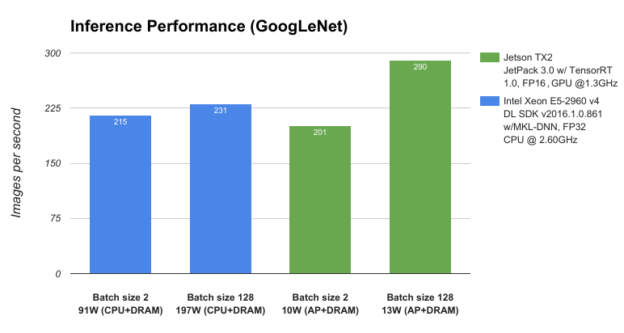
\includegraphics[width=0.6\linewidth]{img/google-net.png}
                \caption{Performance of GoogLeNet network architecture profiled on NVIDIA Jetson TX2 and Intel Xeon E5-2960 v4}
            \end{figure}
            This exceptional AI performance and efficiency of Jetson TX2 stems from the new Pascal GPU architecture and dynamic energy profiles (Max-Q and Max-P), optimized deep learning libraries that come with JetPack 3.0, and the availability of large memory bandwidth.
        \subsubsection{Max-Q and Max-P}
            Jetson TX2 was designed for peak processing efficiency at 7.5W of power. This level of performance, referred to as Max-Q, represents the peak of the power/throughput curve. Every component on the module including the power supply is optimized to provide highest efficiency at this point. 
            The Max-Q frequency for the GPU is 854 MHz, and for the Arm A57 CPUs it’s 1.2 GHz. The L4T BSP in JetPack 3.0 includes preset platform configurations for setting Jetson TX2 in Max-Q mode. JetPack 3.0 also includes a new command line tool called \textbf{nvpmodel} for switching profiles at run time. 
            While Dynamic Voltage and Frequency Scaling (DVFS) permits Jetson TX2’s Tegra “Parker” SoC to adjust clock speeds at run time according to user load and power consumption, the Max-Q configuration sets a cap on the clocks to ensure that the application is operating in the most efficient 
            range only. The table below here shows the performance and energy efficiency of Jetson TX2 and Jetson TX1 when running the GoogLeNet and AlexNet deep learning benchmarks. The performance of Jetson TX2 operating in Max-Q mode is similar to the performance of Jetson TX1 operating at maximum 
            clock frequency but consumes only half the power, resulting in double the energy efficiency. \\ 
            \vspace{3mm}
            Although most platforms with a limited power budget will benefit most from Max-Q behavior, others may prefer maximum clocks to attain peak throughput, albeit with higher power consumption and reduced efficiency. DVFS can be configured to run at a range of other clock speeds, including 
            underclocking and overclocking. Max-P, the other preset platform configuration, enables maximum system performance in less than 15W. The Max-P frequency is 1122 MHz for the GPU and 2 GHz for the CPU when either Arm A57 cluster is enabled or Denver 2 cluster is enabled and 1.4 GHz when 
            both the clusters are enabled. You can also create custom platform configurations with intermediate frequency targets to allow balancing between peak efficiency and peak performance for your application.
            \begin{figure}[H]
                \centering
                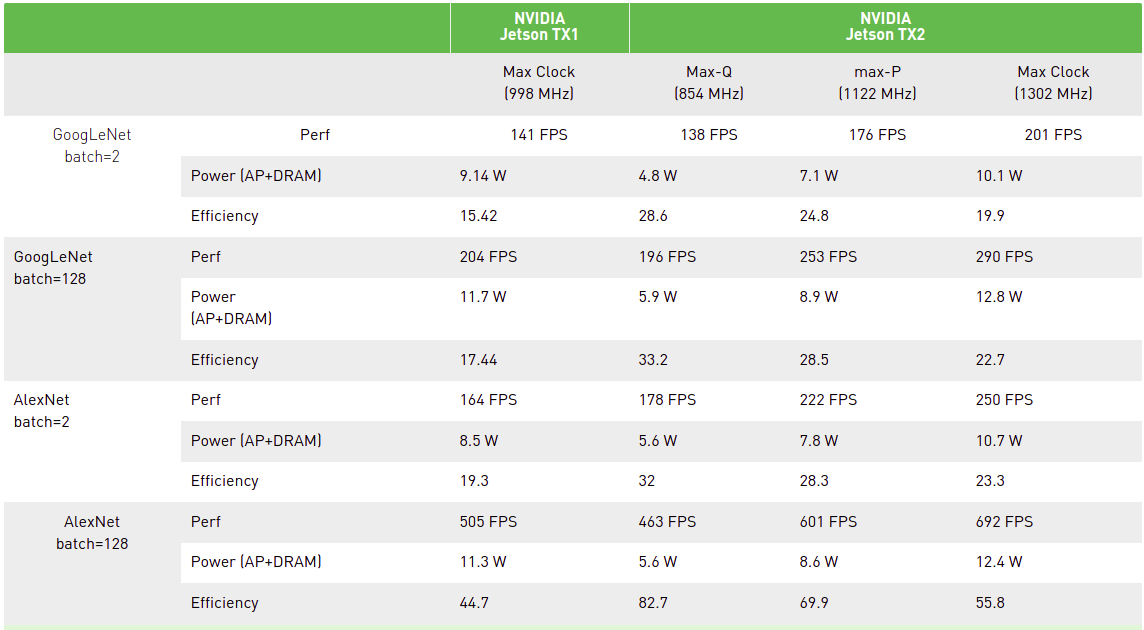
\includegraphics[width=0.6\linewidth]{img/AletNet.png}
                \caption{Power consumption measurements for GoogLeNet and AlexNet architectures for max-Q and max-P performance levels on NVIDIA Jetson TX1 and Jetson TX2. The table reports energy efficiency for all tests in images per second per Watt consumed}
            \end{figure}
            Jetson TX2 performs GoogLeNet inference up to 33.2 images/sec/Watt, nearly double the efficiency of Jetson TX1 and nearly 20X more efficient than Intel Xeon.
        \subsubsection{End-to-End AI Applications}
            Integral to Jetson TX2’s efficient performance are two \textbf{Pascal Streaming Multiprocessors (SMs)} with 128 CUDA cores each. The Pascal GPU architecture offers major performance improvements and power optimizations. TX2’s CPU Complex includes a dual-core 7-way superscalar 
            NVIDIA Denver 2 for high single-thread performance with dynamic code optimization, and a quad-core Arm Cortex-A57 geared for multithreading. \\ 
            \vspace{3mm}
            The coherent Denver 2 and A57 CPUs each have a 2MB L2 cache and are linked via high-performance interconnect fabric designed by NVIDIA to enable simultaneous operation of both CPUs within a Heterogeneous Multiprocessor (HMP) environment. The coherency mechanism allows tasks 
            to be freely migrated according to dynamic performance needs, efficiently utilizing resources between the CPU cores with reduced overhead. \\ 
            \vspace{3mm}
            \textbf{Jetson TX2} is the ideal platform for the end-to-end AI pipeline for autonomous machines. Jetson is wired for streaming live high-bandwidth data: it can simultaneously ingest data from multiple sensors and perform media decoding/encoding, networking, and low-level command \& control 
            protocols after processing the data on the GPU. Figure below here showns common pipeline configurations with sensors attached using an array of high-speed interfaces including CSI, PCIe, USB3, and Gigabit Ethernet. The CUDA pre- and post-processing stages generally consist of 
            colorspace conversion (imaging DNNs typically use BGR planar format) and statistical analysis of the network outputs.
            \begin{figure}[H]
                \centering
                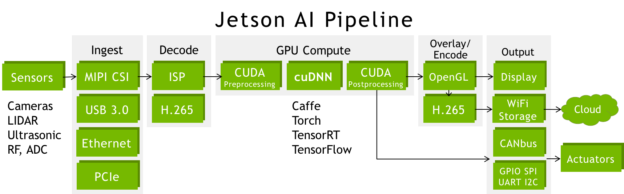
\includegraphics[width=0.6\linewidth]{img/AI-pipeline.png}
                \caption{End-to-end AI pipeline including sensor acquisition, processing, command \& control}
            \end{figure}
            With double the memory and bandwidth than Jetson TX1, Jetson TX2 is able to capture and process additional streams of high-bandwidth data simultaneously, including stereo cameras and 4K ultra-HD inputs and outputs. Through the pipeline deep learning and computer vision fuse together 
            multiple sensors from varying sources and spectral domains, increasing perception and situational awareness during autonomous navigation.
        \subsubsection{Jetson TX2 Developer Kit}
            NVIDIA provides the Jetson TX2 Developer Kit complete with a reference mini-ITX carrier board (170 mm x 170mm) and a 5-megapixel MIPI CSI-2 camera module. The Developer Kit includes documentation and design schematics and free software updates to JetPack-L4T. Down here is the picture of 
            the development kit, showing the Jetson TX2 module and standard PC connections including USB3, HDMI, RJ45 Gigabit Ethernet, SD card, and a PCIe x4 slot, which make it easy to develop applications for Jetson.
            \begin{figure}[H]
                \centering
                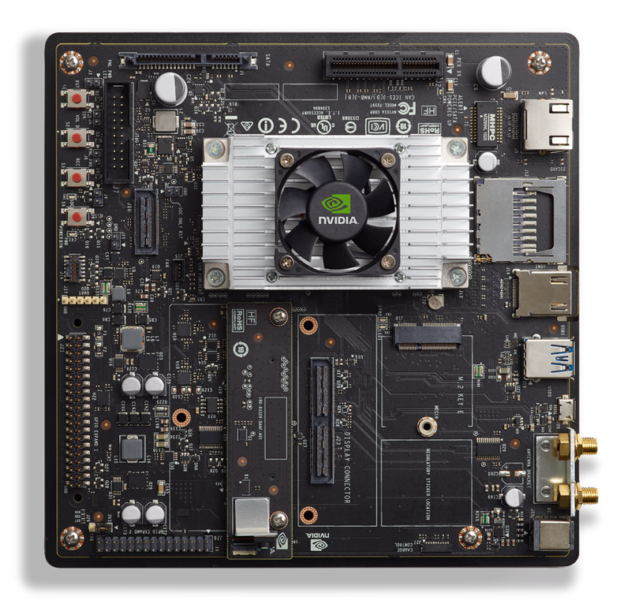
\includegraphics[width=0.6\linewidth]{img/tx2-dev-kit.png}
                \caption{NVIDIA Jetson TX2 Developer Kit including module, reference carrier, and camera module}
            \end{figure}
            To move beyond development to custom deployed platforms, you can modify the reference design files for the Developer Kit carrier board and camera module to create a custom design. Alternatively, Jetson ecosystem partners offer off-the-shelf solutions for deploying Jetson TX1 and 
            Jetson TX2 modules, including miniature carriers, enclosures, and cameras.
